\documentclass[twocolumn,10pt]{article}

% ---- Packages ----
\usepackage{amsmath,amssymb,amsfonts}
\usepackage{booktabs}
\usepackage{graphicx}
\usepackage{xcolor}
\usepackage{hyperref}
\usepackage[margin=0.75in]{geometry}
\usepackage{caption}
\usepackage{natbib}
\bibliographystyle{plainnat}
\usepackage{authblk}
\usepackage[T1]{fontenc}
\usepackage{microtype}
\usepackage{enumitem}
\setlist{nosep,leftmargin=*}

% ---- Metadata ----
\title{\textbf{The Parasitic Channel: An Information-Theoretic Measurement of Immune Evasion Across Three Parasite Systems}}

\author[1]{Lennart Lopin\thanks{ORCID: 0009-0001-2751-2060. Correspondence: lennart@eulersidentity.io}}
\affil[1]{Euler's Identity LLC}

\date{April 2026}

\begin{document}
\maketitle
\thispagestyle{empty}

% ============================================================
% ABSTRACT
% ============================================================
\begin{abstract}
We present the first empirical measurement of parasitic immune evasion in Shannon's information-theoretic framework.  Modeling the immune system as a communication channel---with pathogen molecular identity as the source signal, immune signaling cascades as the channel, and effector response as the output---we compute the Shannon entropy of antigenic repertoires from three independent parasite systems and compare each against published measurements of immune channel capacity.  \textit{Plasmodium falciparum} deploys 3,249 distinct var gene domain architectures across 2,398 clinical isolates \citep{otto2019}, producing a global antigenic entropy of $H = 6.79$~bits [95\% CI: 6.76, 6.79]---$7.4\times$ the measured capacity of the NF-$\kappa$B signaling pathway ($C = 0.92$~bits, \citealt{cheong2011}).  \textit{Trypanosoma brucei} VSG expression entropy oscillates between 0.04 and 3.99 bits over the course of infection \citep{mugnier2015}, crossing above and below the immune channel capacity threshold as the host clears dominant variants and the parasite switches---the Shannon limit made visible in real-time infection dynamics.  HIV-1 envelope protein entropy averages 2.98 bits per residue position [2.94, 3.03] across 496 sequences, with 99.5\% of positions exceeding the 0.92-bit NF-$\kappa$B capacity.  All three systems, across all resolution levels analyzed, produce antigenic source entropy that exceeds the immune channel's capacity to discriminate---placing the immune system in Shannon's $R > C$ regime where classification errors are guaranteed.  We argue that this finding is not coincidental but evolutionarily favored: the arbitrarily varying channel (AVC) theorem establishes that any channel with positive capacity \emph{can} be driven to zero capacity by a sufficiently powerful adversary, and evolutionary game theory establishes that natural selection exerts pressure toward capacity-defeating strategies when the genetic repertoire permits them.  The independent evolution of $H > C$ strategies in three phylogenetically unrelated lineages (Apicomplexa, Kinetoplastida, Retroviridae) is consistent with strong convergent selection pressure rather than coincidence.  We address the principal objection---that the immune system is a massively parallel, adaptive network rather than a single NF-$\kappa$B wire---by deriving multi-receiver capacity bounds and formalizing the rate-of-novelty versus rate-of-learning comparison using the \textit{T.~brucei} temporal data.  The core finding ($H > C$ at the per-interaction level) survives these corrections; the theoretical implications require careful qualification.
\end{abstract}

\smallskip
\noindent\textbf{Keywords:} information theory, Shannon entropy, channel capacity, parasitology, immune evasion, antigenic variation, arbitrarily varying channel, evolutionary game theory

% ============================================================
% 1. INTRODUCTION
% ============================================================
\section{Introduction}
\label{sec:intro}

Every communication channel is a vulnerability.

The claim follows directly from Shannon's noisy channel coding theorem~\citep{shannon1948}.  A channel with positive capacity $C > 0$ can transmit information reliably---but only if the noise is stochastic, not adversarial.  When an adversary can choose the noise, the arbitrarily varying channel (AVC) framework \citep{blackwell1960,csiszar1988} shows that capacity can be driven to \emph{exactly zero} if the adversary achieves ``symmetrizability''---the ability to perfectly mimic legitimate signals.  No biological parasite achieves perfect symmetrizability; molecular mimicry is always imperfect, and the immune system exploits invariant epitopes, conserved binding domains, and pathogen-associated molecular patterns that cannot be disguised without loss of function.  But the AVC framework establishes the \emph{direction} of evolutionary pressure: any strategy that moves toward symmetrizability---that increases antigenic entropy relative to channel capacity---is favored.

Biological immune systems function as communication channels.  The source signal is the molecular identity of encountered entities (self vs.\ non-self, dangerous vs.\ safe).  The channel is the intracellular signaling cascade that transduces antigen recognition into effector response.  The capacity of this channel has been measured: the TNF$\to$NF-$\kappa$B pathway transmits $0.92 \pm 0.01$ bits per cell at a single timepoint~\citep{cheong2011}, dynamic encoding raises this to ${\sim}1.5$~bits~\citep{selimkhanov2014}, and six distinct NF-$\kappa$B ``signaling codons'' achieve ${\sim}2.6$~bits~\citep{adelaja2021}.  All three values are Shannon mutual information computed from single-cell data using standard information-theoretic definitions.

Parasites are adversarial noise sources that exploit these channels.  This paper measures the exploitation.  We compute the Shannon entropy of antigenic repertoires from three independent parasite systems---\textit{Plasmodium falciparum}, \textit{Trypanosoma brucei}, and HIV-1---and compare each against published immune channel capacity measurements.  The fundamental question is whether parasitic antigenic diversity exceeds the immune system's information-processing capacity---whether parasites force the immune recognition system into Shannon's $R > C$ regime where reliable decoding is impossible.

To our knowledge, no prior work has computed the Shannon entropy of antigenic variation and compared it to measured immune signaling capacity as a direct test of information-theoretic limits.  The parasitology literature describes evasion mechanisms in molecular detail.  The systems biology literature measures immune channel capacity.  But the two have not been connected: nobody has asked whether the parasite's source entropy exceeds the channel's capacity, and what that inequality implies under Shannon's theorem.

We find that it does---consistently, across three independent systems, at every resolution level analyzed.

\subsection{Structure of the Paper}

Section~\ref{sec:related} reviews the three literatures our contribution bridges: immune signaling as information processing, parasitic immune evasion, and the AVC/game-theoretic framework.  Section~\ref{sec:framework} presents the formal framework: the immune recognition channel model, Shannon entropy and channel capacity, and the AVC inevitability argument.  Section~\ref{sec:data} describes the data and methods.  Section~\ref{sec:results} presents results from three independent parasite systems.  Section~\ref{sec:why} develops the inevitability argument connecting AVC theory, evolutionary game theory, and the empirical findings.  Section~\ref{sec:discussion} discusses limitations, implications, and future directions.

% ============================================================
% 2. RELATED WORK
% ============================================================
\section{Related Work}
\label{sec:related}

\subsection{The Immune System as an Information Channel}

The application of Shannon's information theory to cellular signaling has produced a decade of rigorous measurements.  \citet{cheong2011} computed the channel capacity of the TNF$\to$NF-$\kappa$B pathway at $0.92 \pm 0.01$~bits per cell---barely sufficient for binary discrimination between ``TNF present'' and ``TNF absent.''  \citet{selimkhanov2014} showed that dynamic encoding through temporal patterns raises capacity to ${\sim}1.5$~bits.  \citet{uda2013} measured ${\sim}1$~bit for growth factor signaling through ERK, Akt, and S6 pathways.  \citet{adelaja2021} identified six distinct NF-$\kappa$B ``signaling codons'' (speed, peak, duration, total, early-vs-late, oscillation) achieving ${\sim}2.6$~bits.  Most recently, \citet{nalecz2023} demonstrated that pulsatile temporal encoding through the MAPK/ERK pathway achieves $\geq 6$~bits/hour.

For immune recognition specifically, \citet{ganti2020} showed that T-cell receptor (TCR) discrimination capacity increases across the kinetic proofreading cascade: ${\sim}0.07$~bits after initial Lck recruitment, increasing to ${\sim}1$~bit after full LAT phosphorylation.  The realized TCR repertoire diversity in young adults comprises approximately $10^8$ unique TCR$\beta$ sequences (${\sim}26.6$~bits of combinatorial diversity), but the per-interaction channel capacity---how much a single TCR engagement tells the cell about antigen identity---remains near 1~bit.

These measurements establish that immune signaling channels operate near their capacity limits.  Any parasitic interference that reduces capacity, or any parasitic diversity that exceeds capacity, pushes the system below the threshold for reliable discrimination.

\subsection{Parasitic Immune Evasion}

The molecular mechanisms of parasitic immune evasion are extensively documented but have never been quantified information-theoretically.

\textit{Plasmodium falciparum} encodes ${\sim}60$ var genes per genome, each encoding a distinct PfEMP1 surface protein.  Only one is expressed at a time, with stochastic switching at rates of ${\sim}2\%$ per generation~\citep{horrocks2004}.  Population-level surveys identify thousands of distinct variants with minimal overlap between geographic populations~\citep{barry2007,day2017,otto2019}.

\textit{Trypanosoma brucei} maintains ${\sim}2{,}500$ VSG genes per genome, with ${\sim}20\%$ potentially functional.  \citet{mugnier2015} used VSG-seq to track in vivo switching dynamics, finding that up to 100 VSGs are expressed simultaneously and that the repertoire is explored sequentially over months-long infections.

HIV-1 mutates at $3.4 \times 10^{-5}$ per nucleotide per replication cycle, generating continuous antigenic novelty.  The envelope glycoprotein (env/gp160) is the primary target of neutralizing antibodies and the most variable protein in the HIV genome.

All three systems have been studied with evolutionary game theory~\citep{bremermann1983,nowak1994,frank1996}, but never with Shannon's information theory.  The game-theoretic literature asks what strategy the parasite \emph{should} adopt; we ask how much information the parasite's strategy \emph{destroys}.

\subsection{The Gap}

\citet{bellamy2024} model immune-pathogen coevolution using entropy production and information exchange rates, introducing ``co-evolutionary efficiency.''  \citet{mora2023} argue that a quantitative theory of viral-immune coevolution is within reach.  \citet{bergstrom2005} proved that the fitness value of environmental information equals the mutual information between cue and environment.  These works approach the intersection of information theory and immunology but do not measure antigenic entropy against immune channel capacity.  \citet{rahman2011} catalog pathogen subversion of NF-$\kappa$B---the very pathway whose channel capacity has been measured---but do not quantify the capacity reduction.  The synthesis we present---computing parasitic source entropy and comparing it to measured channel capacity as a direct test of Shannon's theorem---has not been performed.

% ============================================================
% 3. FORMAL FRAMEWORK
% ============================================================
\section{Formal Framework}
\label{sec:framework}

\subsection{The Immune Recognition Channel}

We model immune recognition as a discrete channel in Shannon's framework.  Define:
\begin{itemize}
\item \textbf{Source $X$:} The antigenic identity of an encountered entity, drawn from an antigenic alphabet $\mathcal{X}$.  For \textit{P.~falciparum}, $\mathcal{X}$ is the set of PfEMP1 domain architectures.  For \textit{T.~brucei}, $\mathcal{X}$ is the set of expressed VSG variants.  For HIV, $\mathcal{X}$ is the set of env protein sequences.
\item \textbf{Channel $P(Y|X)$:} The immune signaling cascade that transduces antigen recognition into effector output.  Characterized by the conditional distribution of immune response $Y$ given antigen $X$.
\item \textbf{Output $Y$:} The effector response---cytokine production, T-cell activation, antibody secretion, or the binary decision: attack or tolerate.
\item \textbf{Channel capacity:}
\begin{equation}
C = \max_{P(X)} I(X;Y) = \max_{P(X)} \sum_{x,y} P(x,y) \log_2 \frac{P(x,y)}{P(x)P(y)}
\label{eq:capacity}
\end{equation}
\end{itemize}

\subsection{Shannon Entropy of Antigenic Repertoires}

The Shannon entropy of the antigenic source distribution is:
\begin{equation}
H(X) = -\sum_{x \in \mathcal{X}} P(x) \log_2 P(x)
\label{eq:entropy}
\end{equation}
This measures the information content (in bits) of the antigenic signal the immune system must decode.  For a repertoire of $K$ equally likely types, $H(X) = \log_2 K$.  For non-uniform distributions, $H(X) < \log_2 K$.

\subsection{The Shannon Limit in Immune Recognition}

Shannon's noisy channel coding theorem~\citep{shannon1948} establishes that reliable communication is possible if and only if the transmission rate $R$ satisfies $R \leq C$.  When $R > C$, the probability of decoding error is bounded away from zero---no encoding strategy can achieve reliable discrimination.

In the immune context: if the antigenic entropy $H(X)$ exceeds the immune channel capacity $C$, then the immune system cannot reliably discriminate among all antigenic variants simultaneously.  Formally, the error probability satisfies:
\begin{equation}
P_e \geq 1 - \frac{C + 1}{H(X)}
\label{eq:fano}
\end{equation}
for any decoding strategy (Fano's inequality).  When $H(X) \gg C$, most antigenic variants are indistinguishable to the immune system at any given time.

The immune system can still discriminate among a subset of $2^C$ variants per channel use, and sequential learning (affinity maturation, memory cells) allows the effective capacity to accumulate over multiple encounters.  But at any given moment, the number of simultaneously discriminable variants is bounded by $2^C$, and if the parasite presents more diversity than this, some variants will evade recognition.

\subsection{The Inevitability of Adversarial Channel Degradation}

The arbitrarily varying channel (AVC)~\citep{blackwell1960} provides the game-theoretic foundation.  An AVC is defined by a family $\{W(y|x,s) : s \in \mathcal{S}\}$, where an adversary (the parasite) chooses a state sequence $s^n$ to maximize decoding error, while the encoder-decoder team (the immune system) designs codes to minimize it.

\begin{quote}
\textbf{Theorem} \citep{csiszar1988}.  The deterministic-code capacity of an AVC satisfies a dichotomy: it equals the random-coding capacity $C_{\text{random}} = \max_{P(X)} \min_{q(S)} I(X;Y)$ if the AVC is non-symmetrizable, and equals exactly zero if the AVC is symmetrizable---i.e., if there exists a conditional distribution $\sigma(s|x)$ such that the adversary can perfectly mimic any legitimate codeword.
\end{quote}

The biological interpretation requires careful qualification.  A parasite that achieves full symmetrizability would make its antigens perfectly indistinguishable from self---driving immune capacity to zero.  No biological parasite achieves this.  Molecular mimicry is always imperfect: invariant epitopes, conserved structural motifs, and pathogen-associated molecular patterns (PAMPs such as LPS, flagellin, unmethylated CpG DNA) provide ``side information'' that the immune system exploits, and which the parasite cannot disguise without losing essential biological functions.  Symmetrizability is therefore best understood as an \emph{asymptotic limit} that evolution pushes toward but never reaches---a horizon that shapes the direction of selection without being attained.  The measured $H > C$ finding indicates that parasites have achieved a state far along this trajectory: not perfect symmetrizability, but sufficient antigenic entropy to overwhelm the per-interaction capacity of immune signaling channels.

\subsection{Evolutionary Game Theory: From Possibility to Selection Pressure}

The AVC framework establishes that adversarial channel degradation is \emph{mathematically possible}.  Evolutionary game theory establishes that natural selection \emph{exerts pressure} toward capacity-exceeding strategies---though whether any given organism reaches that state depends on contingent biology.

\citet{bremermann1983} showed that parasite virulence evolves to a Nash equilibrium determined by the host-parasite transmission-virulence tradeoff.  \citet{nowak1994} proved that superinfection creates a Prisoner's Dilemma driving virulence above the cooperative optimum.  \citet{frank1996} connected kin selection to virulence evolution through cooperative game theory.  Forty years of validated results establish that parasites evolve strategies that maximize fitness under evolutionary pressure.

\citet{bergstrom2005} proved the critical connecting result: the fitness value of environmental information equals the mutual information $I(X;Y)$ between environmental cue and environmental state.  In our context: the fitness value of immune recognition equals the mutual information between antigen and immune response.  A parasite that reduces this MI---by increasing antigenic entropy beyond channel capacity---directly reduces the fitness value of the immune system's information channel.

\citet{chastain2014} proved that natural selection under sexual recombination is mathematically equivalent to the Multiplicative Weight Updates Algorithm, which maximizes cumulative expected fitness plus entropy.  Evolution is, provably, an information-theoretic optimization algorithm.

The argument is:
\begin{enumerate}
\item Any channel with $C > 0$ can be degraded by an adversary (AVC theorem---mathematical possibility)
\item Natural selection favors strategies that increase fitness (evolutionary game theory)
\item Reducing immune MI increases parasite fitness (Bergstrom-Lachmann)
\item Therefore, natural selection exerts pressure toward capacity-exceeding antigenic strategies
\end{enumerate}

Many parasites adopt alternative strategies---intracellular hiding, rapid reproduction and transmission before clearance, or direct immunosuppression---that do not require large antigenic repertoires.  The claim is narrower: antigenic variation, \emph{when it evolves}, will be driven toward the $H > C$ regime.  The independent evolution of this strategy in three phylogenetically unrelated lineages is consistent with strong selection pressure, though it does not constitute proof of inevitability in the strict mathematical sense.

% ============================================================
% 4. DATA AND METHODS
% ============================================================
\section{Data and Methods}
\label{sec:data}

\subsection{Data Sources}

We analyze three independent datasets spanning three parasite species, three laboratories, and three data types:

\textbf{Dataset~1: \textit{P.~falciparum} var gene repertoires.}  \citet{otto2019} assembled near-complete var gene repertoires from 2,398 clinical isolates across 18 countries, containing 168,738 var genes with domain architecture annotations.  Data obtained from varDB (Zenodo: doi:10.5281/zenodo.3549732).

\textbf{Dataset~2: \textit{T.~brucei} VSG expression dynamics.}  \citet{mugnier2015} performed VSG-seq on 4 mice infected with \textit{T.~brucei} EATRO~1125, sampled at 8 timepoints each (days 6--30), plus late-infection data (days 96--105).  VSG expression frequencies (percentage of trypanosome population) from supplementary databases S1--S5.  Reference genome: 3,570 VSG sequences in EATRO1125 VSGdb.

\textbf{Dataset~3: HIV-1 envelope protein sequences.}  500 HIV-1 env protein sequences obtained from NCBI Protein Database (Entrez: txid11676[Organism] AND env[Gene Name]).  Filtered to 496 sequences within 10\% of median length (807 analyzable positions).  Cross-subtype dataset; 80.1\% mean pairwise divergence.

\subsection{Channel Capacity Benchmarks}

We compare antigenic entropy against published immune signaling channel capacity measurements (Table~\ref{tab:benchmarks}):

\begin{table}[t]
\centering
\caption{Published immune signaling channel capacity measurements.  We use $C = 0.92$~bits as the primary benchmark (most conservative, most rigorously measured).}
\label{tab:benchmarks}
\footnotesize
\begin{tabular}{@{}lclc@{}}
\toprule
Pathway & $C$ (bits) & Method & Ref. \\
\midrule
TNF$\to$NF-$\kappa$B (snap.) & $0.92 \pm 0.01$ & Binned MI & \footnotesize{\citeyear{cheong2011}} \\
TNF$\to$NF-$\kappa$B (dyn.) & ${\sim}1.5$ & Dynamic MI & \footnotesize{\citeyear{selimkhanov2014}} \\
NF-$\kappa$B codons & ${\sim}2.6$ & 6 codons & \footnotesize{\citeyear{adelaja2021}} \\
TCR proofreading & ${\sim}1.0$ & Model & \footnotesize{\citeyear{ganti2020}} \\
ERK pathway & ${\sim}1.0$ & Amplitude MI & \footnotesize{\citeyear{uda2013}} \\
MAPK/ERK (pulsatile) & ${\geq}6$/hr & Dynamic MI & \footnotesize{\citeyear{nalecz2023}} \\
\bottomrule
\end{tabular}
\end{table}

\subsection{Estimation Procedure}

For each dataset:
\begin{enumerate}
\item Define the antigenic alphabet $\mathcal{X}$ (var domain architectures, VSG variant identities, or amino acid types at each position).
\item Compute the empirical frequency distribution $\hat{P}(x) = n_x / N$.
\item Compute Shannon entropy $H(X) = -\sum_x \hat{P}(x) \log_2 \hat{P}(x)$ using \texttt{scipy.stats.entropy}.
\item Apply Miller-Madow finite-sample bias correction~\citep{miller1955}: $H_{\text{corrected}} = H_{\text{raw}} - (K-1)/(2N\ln 2)$, where $K = |\mathcal{X}|$ and $N$ is the number of observations.
\item Compute 95\% bootstrap confidence intervals from 1,000 resamples with replacement.
\end{enumerate}

\subsection{Sensitivity Analysis}

For \textit{P.~falciparum}, entropy is computed at three taxonomic resolutions: first domain only (18 types, coarsest), full domain architecture (3,249 types), and normalized subdomains (16,089 types, finest).  For \textit{T.~brucei}, entropy is computed per-mouse and per-timepoint, with biological replication across 4 mice.  For HIV, both full and deduplicated sequence sets are analyzed, and $k$-mer entropy is computed at $k = 5, 7, 9, 11, 13$ to test scaling.

% ============================================================
% 5. RESULTS
% ============================================================
\section{Results}
\label{sec:results}

\subsection{\textit{P.~falciparum}: Antigenic Entropy Exceeds Immune Capacity by 4.9--7.4$\times$}

The global Shannon entropy over 3,249 unique var gene domain architectures across 2,398 isolates is:
\begin{equation}
H(X_{\text{global}}) = 6.79 \text{~bits} \quad [95\%~\text{CI}: 6.76, 6.79]
\end{equation}
This is $7.4\times$ the NF-$\kappa$B channel capacity ($C = 0.92$~bits) and $2.6\times$ the NF-$\kappa$B signaling codon capacity ($C = 2.6$~bits).

The mean per-isolate entropy (within individual genomes) is:
\begin{equation}
H(X_{\text{genome}}) = 4.49 \text{~bits} \quad [4.47, 4.52]
\end{equation}
This is $4.9\times$ the NF-$\kappa$B capacity.  A single \textit{P.~falciparum} genome presents more antigenic diversity than the immune signaling channel can resolve.

Per-country entropy is remarkably consistent: 6.36--6.70~bits across the top~5 countries by sample size (Ghana, Cambodia, Malawi, Tanzania, Laos), with a cross-country mean of 6.08~bits.  Bootstrap confidence intervals are tight, indicating the finding is not driven by sampling noise.

\textbf{Sensitivity to resolution.}  At the coarsest resolution (18 first-domain types), $H = 2.04$~bits---still $2.2\times$ the NF-$\kappa$B capacity.  At the finest resolution (16,089 normalized subdomain types), $H = 12.32$~bits---$13.4\times$ capacity.  The finding is robust: at no resolution level does antigenic entropy fall below channel capacity.

\begin{figure}[t]
\centering
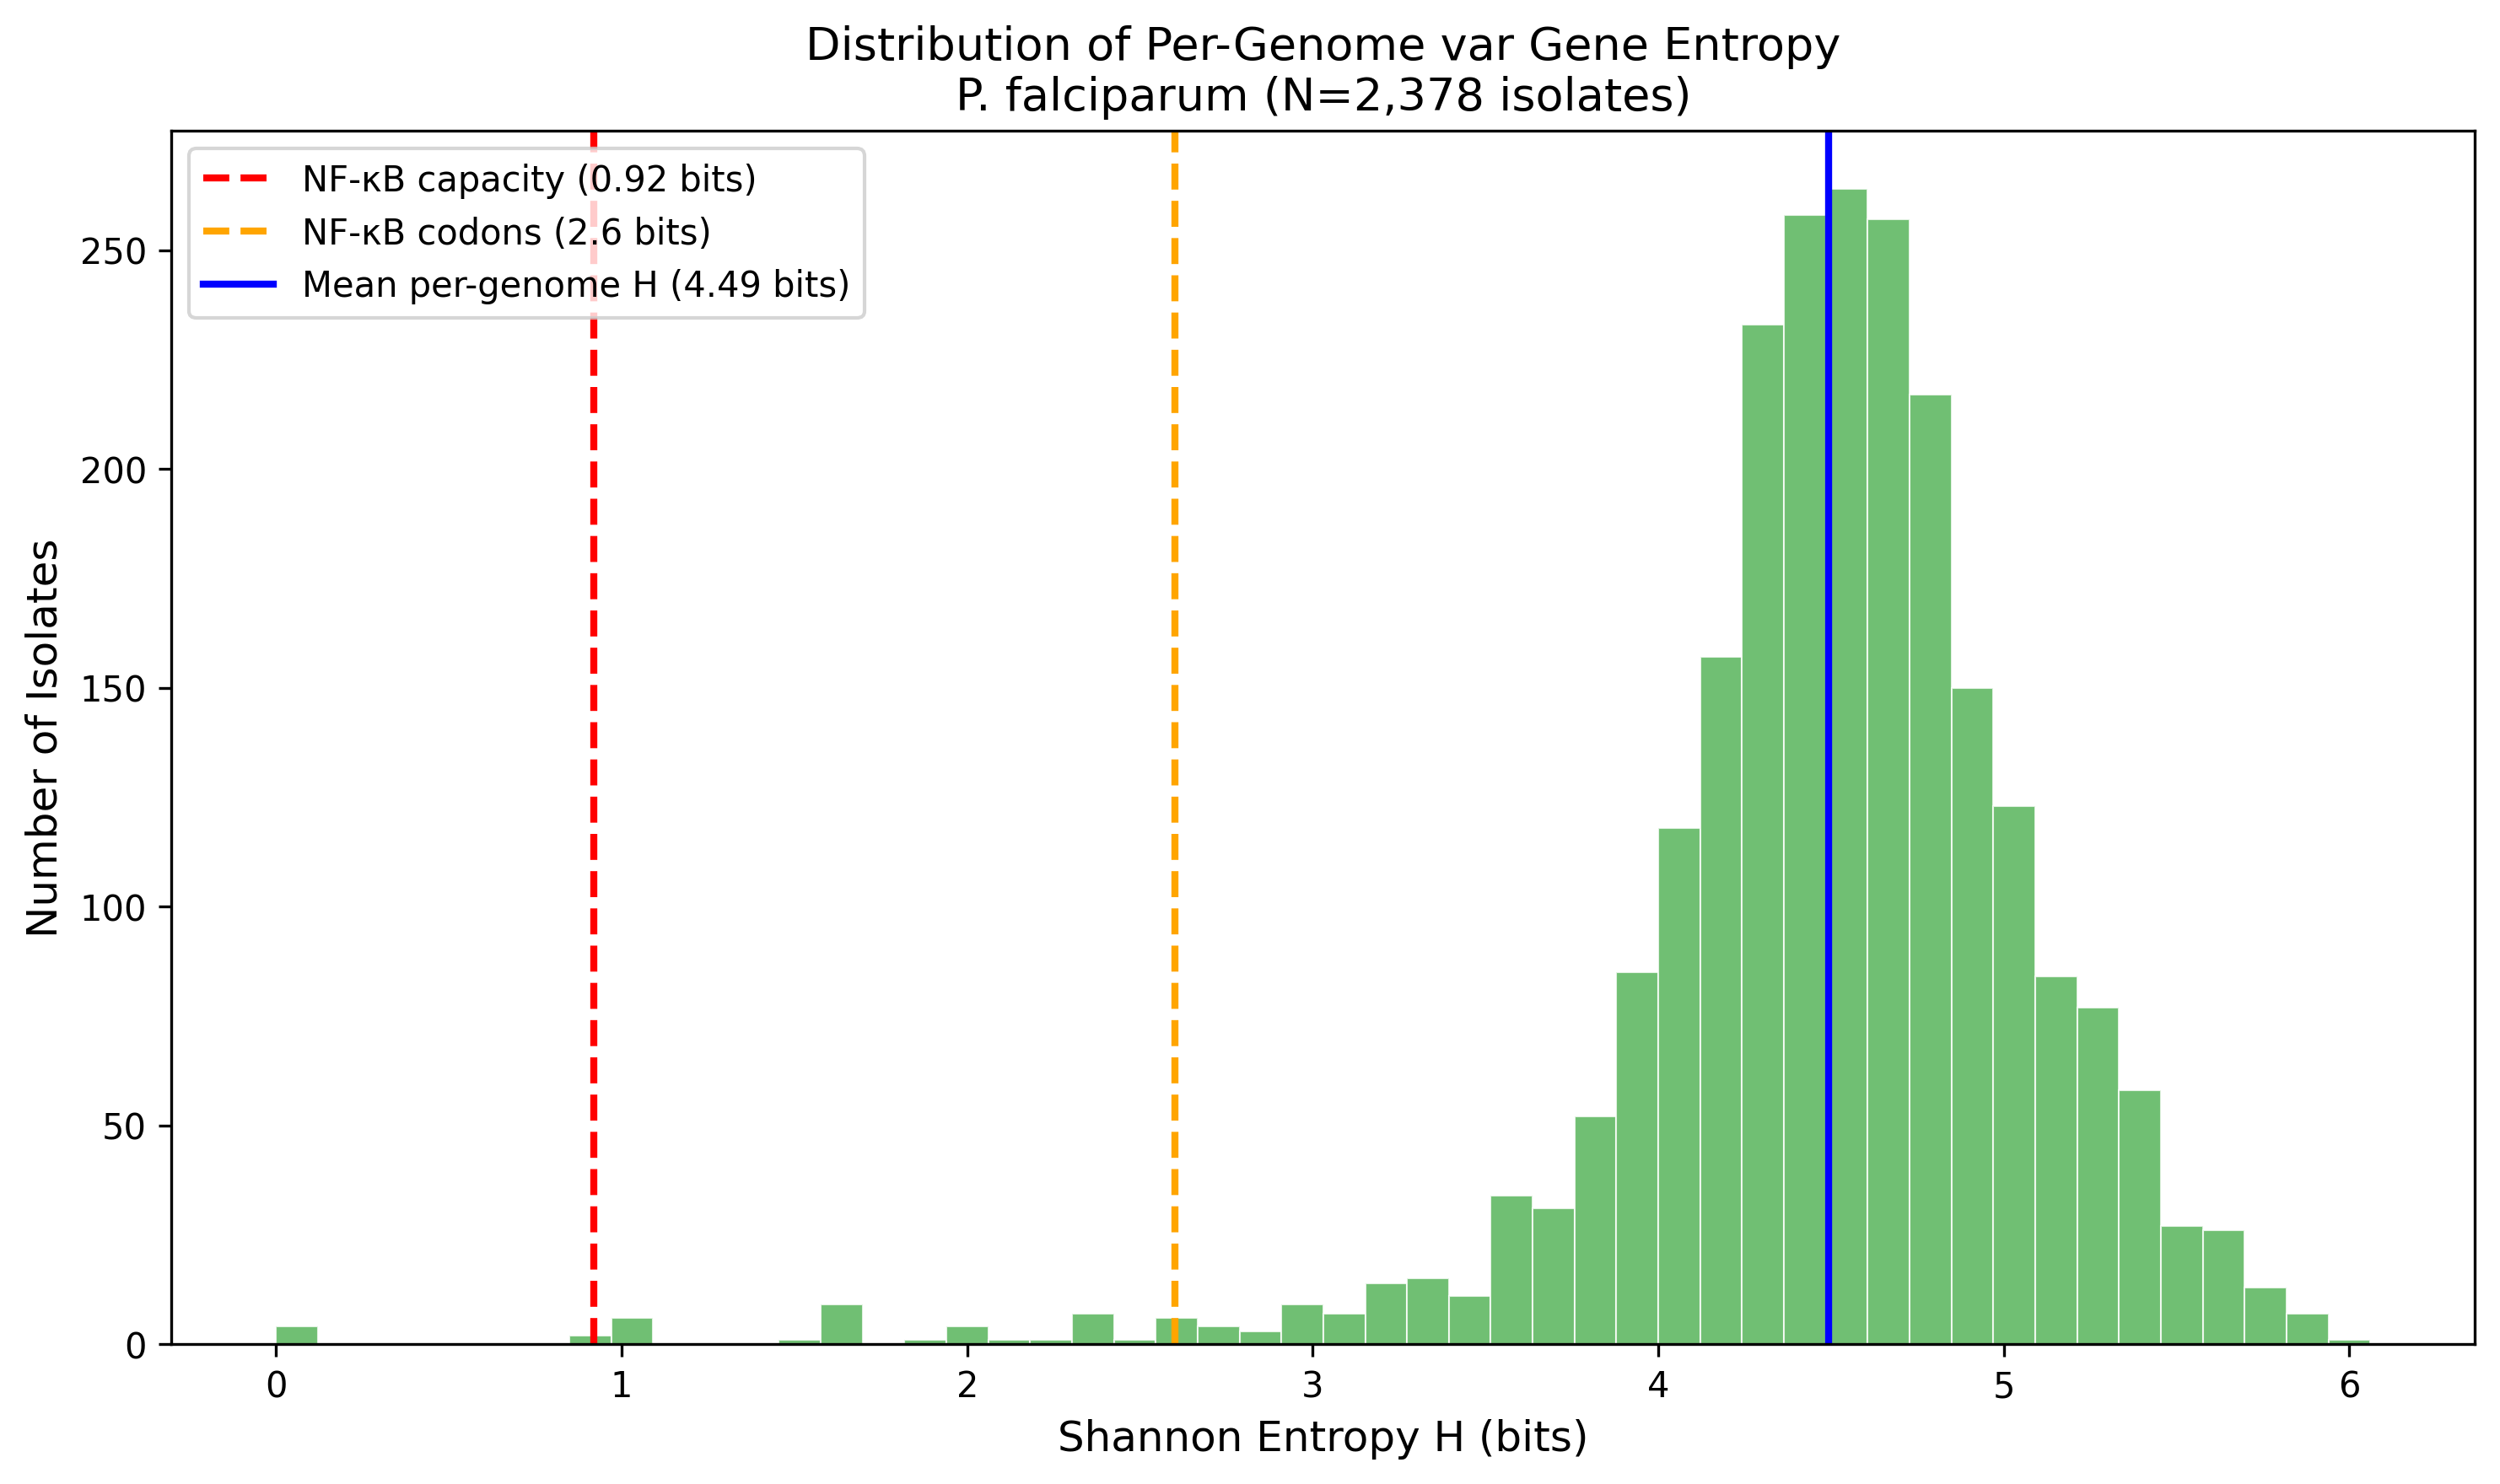
\includegraphics[width=\columnwidth]{figures/fig2_pfalciparum_per_genome_entropy.png}
\caption{Distribution of per-genome antigenic entropy across 2,378 \textit{P.~falciparum} isolates.  Mean $H = 4.49$~bits (blue line) exceeds both the NF-$\kappa$B snapshot capacity (0.92~bits, red) and signaling codon capacity (2.6~bits, orange).  Even within a single parasite genome, antigenic diversity overwhelms the immune channel.}
\label{fig:pergenome}
\end{figure}

\subsection{\textit{T.~brucei}: The Shannon Limit Visible in Real-Time Infection Dynamics}

The mean VSG expression entropy across all 4 mice and 32 mouse-timepoints is:
\begin{equation}
H(X_{\text{VSG}}) = 1.70 \text{~bits} \quad [1.34, 2.07]
\end{equation}
with a maximum single-timepoint entropy of 3.99~bits (Mouse~1, day~26).

The most striking finding is the \emph{temporal trajectory} of entropy.  Rather than increasing monotonically (as would be expected if the parasite simply accumulated diversity), VSG entropy oscillates:
\begin{itemize}
\item \textbf{Days 6--7:} $H \approx 0.04\text{--}0.36$~bits.  A single VSG dominates at 94--99\% of the population.  Entropy is below the 0.92-bit channel capacity.  The immune system can discriminate: it ``sees'' the dominant variant.
\item \textbf{Days 12--18:} $H \approx 1.5\text{--}3.6$~bits.  Multiple VSGs are co-dominant.  Entropy exceeds channel capacity.  The immune system cannot reliably discriminate among variants.
\item \textbf{Day 24:} $H$ drops to ${\approx}0.05\text{--}2.0$~bits.  The immune system has cleared the previously dominant variant; a new dominant emerges.  Entropy briefly drops below capacity again.
\item \textbf{Days 26--30:} $H \approx 0.9\text{--}4.0$~bits.  The cycle repeats.
\end{itemize}

This oscillation is the Shannon limit in action.  When entropy is below $C$, the immune system can identify and clear the dominant variant (reliable decoding).  When entropy exceeds $C$, the immune system cannot distinguish among co-dominant variants (decoding errors), and the parasite population gains time to establish new dominants.  The arms race between host and parasite oscillates around the capacity threshold.

\begin{figure*}[t]
\centering
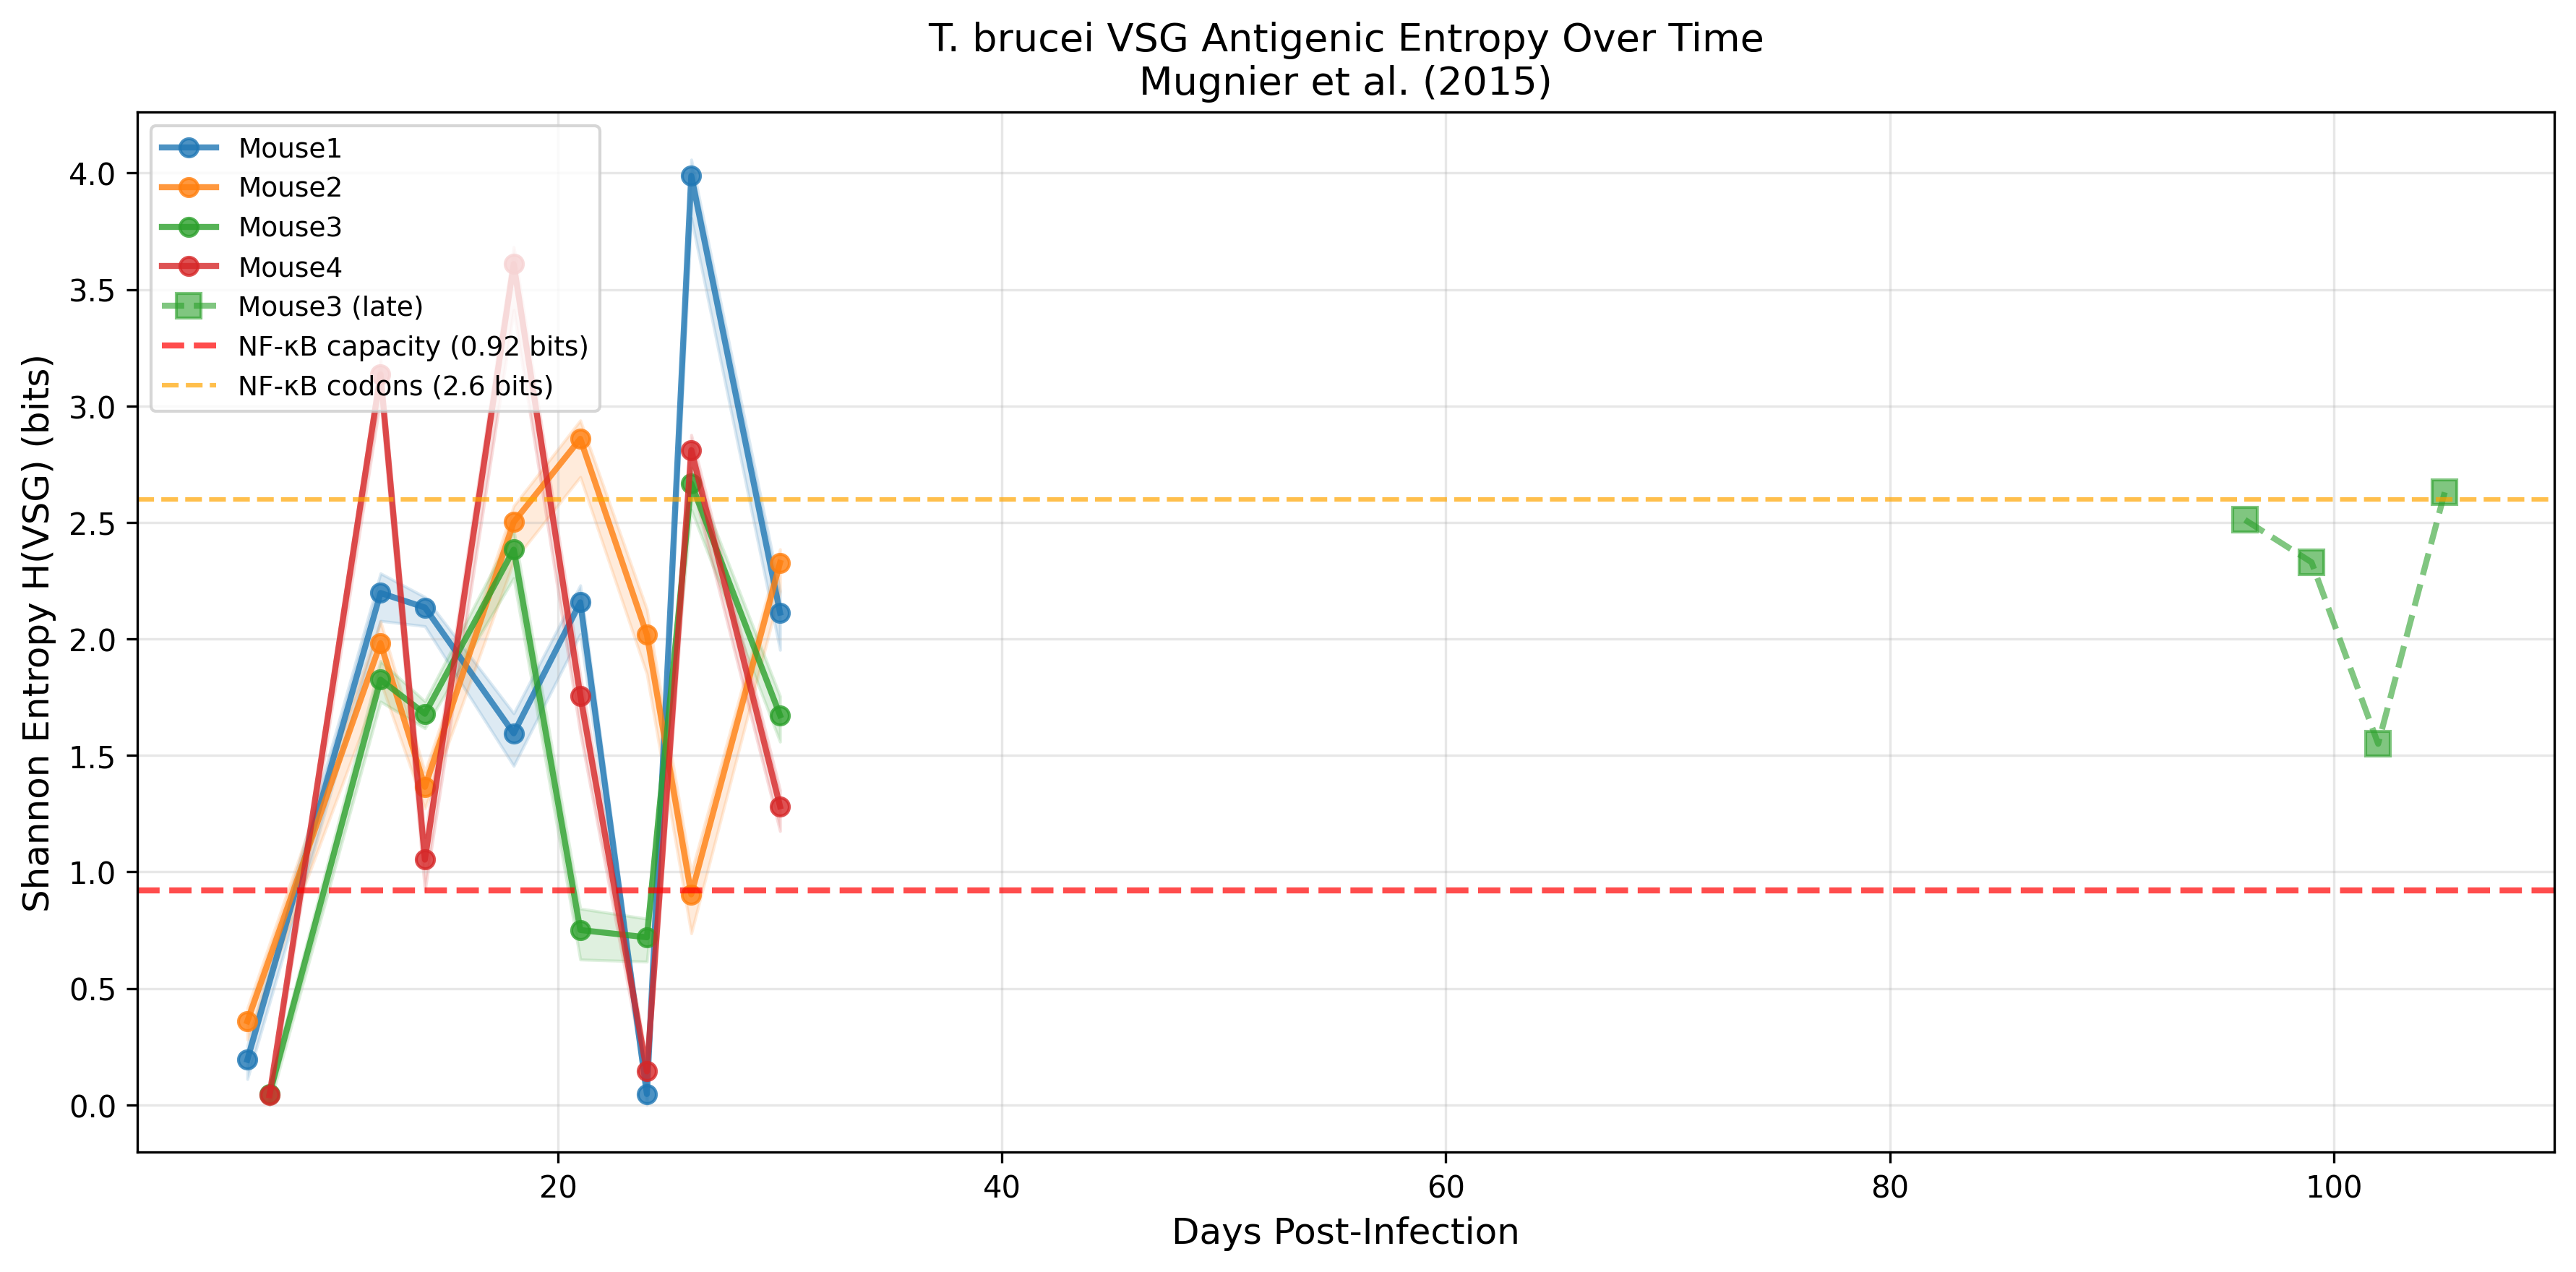
\includegraphics[width=\textwidth]{figures/fig4_tbrucei_entropy_over_time.png}
\caption{VSG expression entropy oscillates above and below the immune channel capacity threshold during \textit{T.~brucei} infection.  Four mice (EATRO~1125 strain) tracked over days 6--30.  Horizontal dashed line: NF-$\kappa$B snapshot capacity ($C = 0.92$~bits, \citealt{cheong2011}).  Entropy crosses the capacity boundary repeatedly as the immune system clears dominant variants and the parasite switches---the Shannon limit made visible in real-time infection dynamics.  Shaded bands: 95\% bootstrap CIs.  Mouse~3 late-infection data (days 96--105) shown at right.}
\label{fig:tbrucei}
\end{figure*}

The mutual information between timepoint and VSG identity is $I(\text{time}; \text{VSG}) = 2.2\text{--}2.6$~bits across mice (87\% of temporal uncertainty resolved).  This confirms that VSG switching is sequential, not random---the parasite deploys its antigenic repertoire in a structured order, consistent with game-theoretic predictions of optimal switching strategies.

\textbf{Biological replication.}  Results are consistent across all 4 mice: Mouse~1 mean $H = 1.80$ [1.00, 2.59]; Mouse~2: 1.79 [1.24, 2.29]; Mouse~3: 1.47 [0.88, 2.07]; Mouse~4: 1.73 [0.85, 2.61].

\textbf{Late infection.}  At days 96--105, entropy is 2.25~bits with 97 distinct VSGs detected---confirming that the parasite maintains above-capacity diversity throughout chronic infection.

\subsection{HIV-1: 99.5\% of Envelope Positions Exceed Immune Channel Capacity}

The mean per-position Shannon entropy of the HIV-1 env protein across 496 sequences and 807 analyzable positions is:
\begin{equation}
H(X_{\text{position}}) = 2.98 \text{~bits} \quad [2.94, 3.03]
\end{equation}
This is $3.2\times$ the NF-$\kappa$B capacity and 69\% of the theoretical maximum ($\log_2 20 = 4.32$~bits per position for 20 amino acids).

\textbf{99.5\% of positions exceed the 0.92-bit NF-$\kappa$B capacity}, and 85\% exceed the 2.6-bit NF-$\kappa$B signaling codon capacity.  The positional entropy profile reveals biologically meaningful structure: positions 1--100 (signal peptide, conserved gp120 core) show lower entropy (1.5--2.5~bits), followed by a sharp increase at positions 100--200 (variable loops V1-V2, peak at 3.81~bits), sustained high entropy through positions 200--800 (gp120 outer domain, V3-V5 loops, gp41).  The concentration of entropy at immune-facing surfaces is consistent with the interpretation that antigenic variation is an evolved information-theoretic strategy targeting the recognition channel.

\begin{figure}[t]
\centering
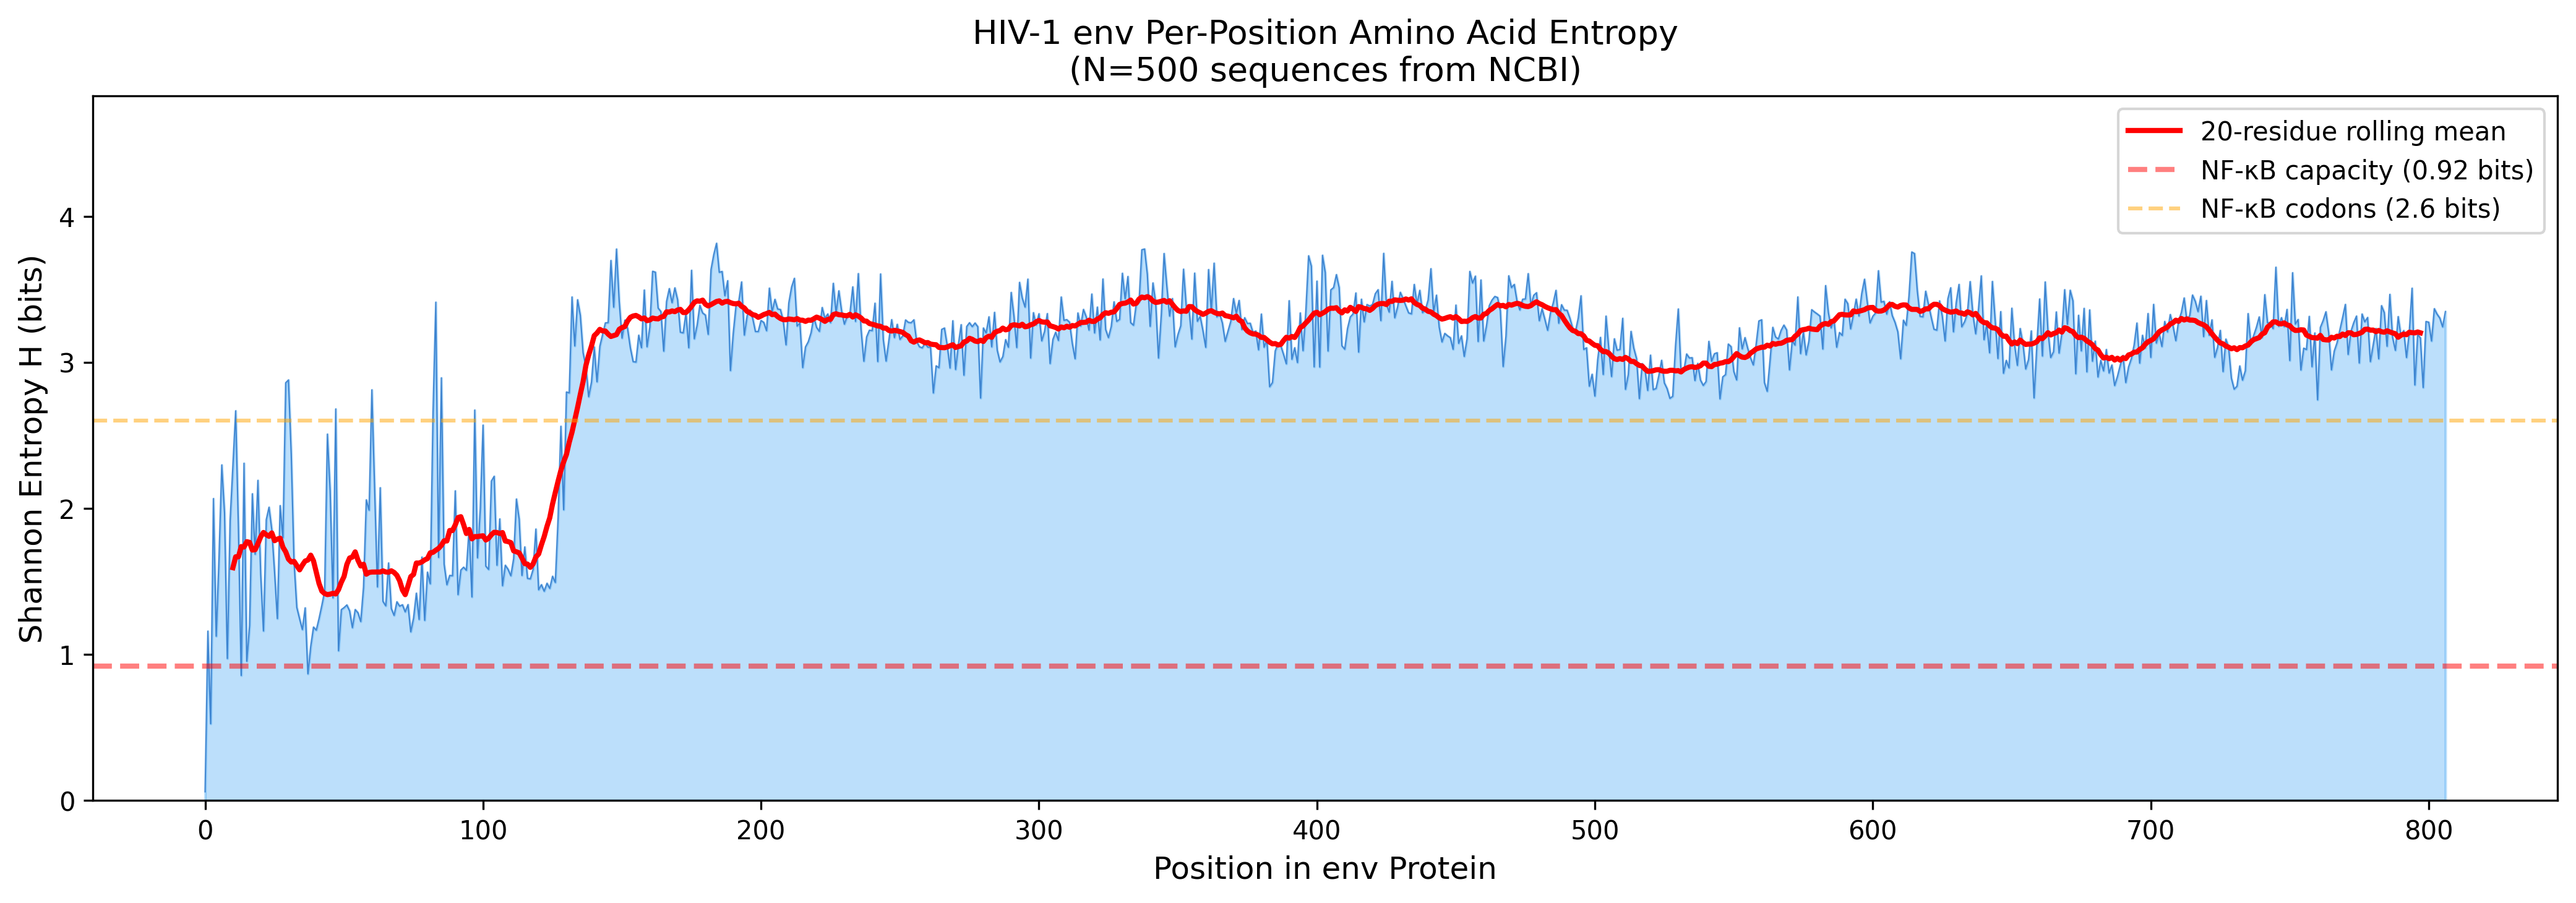
\includegraphics[width=\columnwidth]{figures/fig7_hiv_positional_entropy.png}
\caption{Per-position Shannon entropy along the HIV-1 envelope protein ($N = 496$ sequences).  Positions 100--200 (variable loops V1-V2) show peak entropy.  99.5\% of positions exceed the 0.92-bit NF-$\kappa$B capacity (lower dashed line); 85\% exceed the 2.6-bit signaling codon capacity (upper dashed line).  Red line: 20-residue rolling mean.}
\label{fig:hiv}
\end{figure}

\textbf{$k$-mer epitope entropy} (at MHC-I-relevant 9-mer length) is 13.94~bits [13.75, 13.77] over 81,566 unique 9-mers---$15.1\times$ the NF-$\kappa$B capacity.  Since MHC presentation operates on peptide fragments, the 9-mer entropy is the operationally relevant measure for T-cell recognition.

\textbf{Cross-subtype caveat.}  The 80.1\% mean pairwise divergence confirms the dataset spans multiple HIV-1 subtypes, inflating entropy relative to within-subtype diversity.  We note three mitigations: (1) even a 50\% reduction in mean per-position entropy would yield ${\sim}1.49$~bits, still exceeding the 0.92-bit benchmark; (2) published LANL subtype-B analyses report 1.5--2.0~bits at variable loops, still above capacity; (3) the MHC system encounters cross-subtype diversity when an individual is re-exposed to different viral strains, making the global entropy epidemiologically relevant.

\subsection{Convergence Across Three Systems}

Table~\ref{tab:main} synthesizes the results.  The headline finding:
\begin{equation}
\frac{H_{\text{parasite}}}{C_{\text{immune}}} > 1
\end{equation}
for all systems, all resolutions, and all bootstrap resamples.

\begin{table}[t]
\centering
\caption{Antigenic source entropy vs.\ immune channel capacity across three parasite systems.}
\label{tab:main}
\footnotesize
\begin{tabular}{@{}lrcr@{}}
\toprule
System & $H$ (bits) & 95\% CI & $H/C^*$ \\
\midrule
\textit{P.~f.} per-genome & 4.49 & [4.47, 4.52] & 4.9$\times$ \\
\textit{P.~f.} global (3,249 types) & 6.79 & [6.76, 6.79] & 7.4$\times$ \\
\textit{T.~b.} mean VSG (4 mice) & 1.70 & [1.34, 2.07] & 1.8$\times$ \\
\textit{T.~b.} max timepoint & 3.99 & --- & 4.3$\times$ \\
HIV-1 per-position env & 2.98 & [2.94, 3.03] & 3.2$\times$ \\
HIV-1 9-mer epitope & 13.94 & [13.75, 13.77] & 15.1$\times$ \\
\bottomrule
\end{tabular}
\smallskip

\footnotesize{$^*$$H/C$ computed against $C = 0.92$~bits \citep{cheong2011}.}
\end{table}

\begin{figure}[t]
\centering
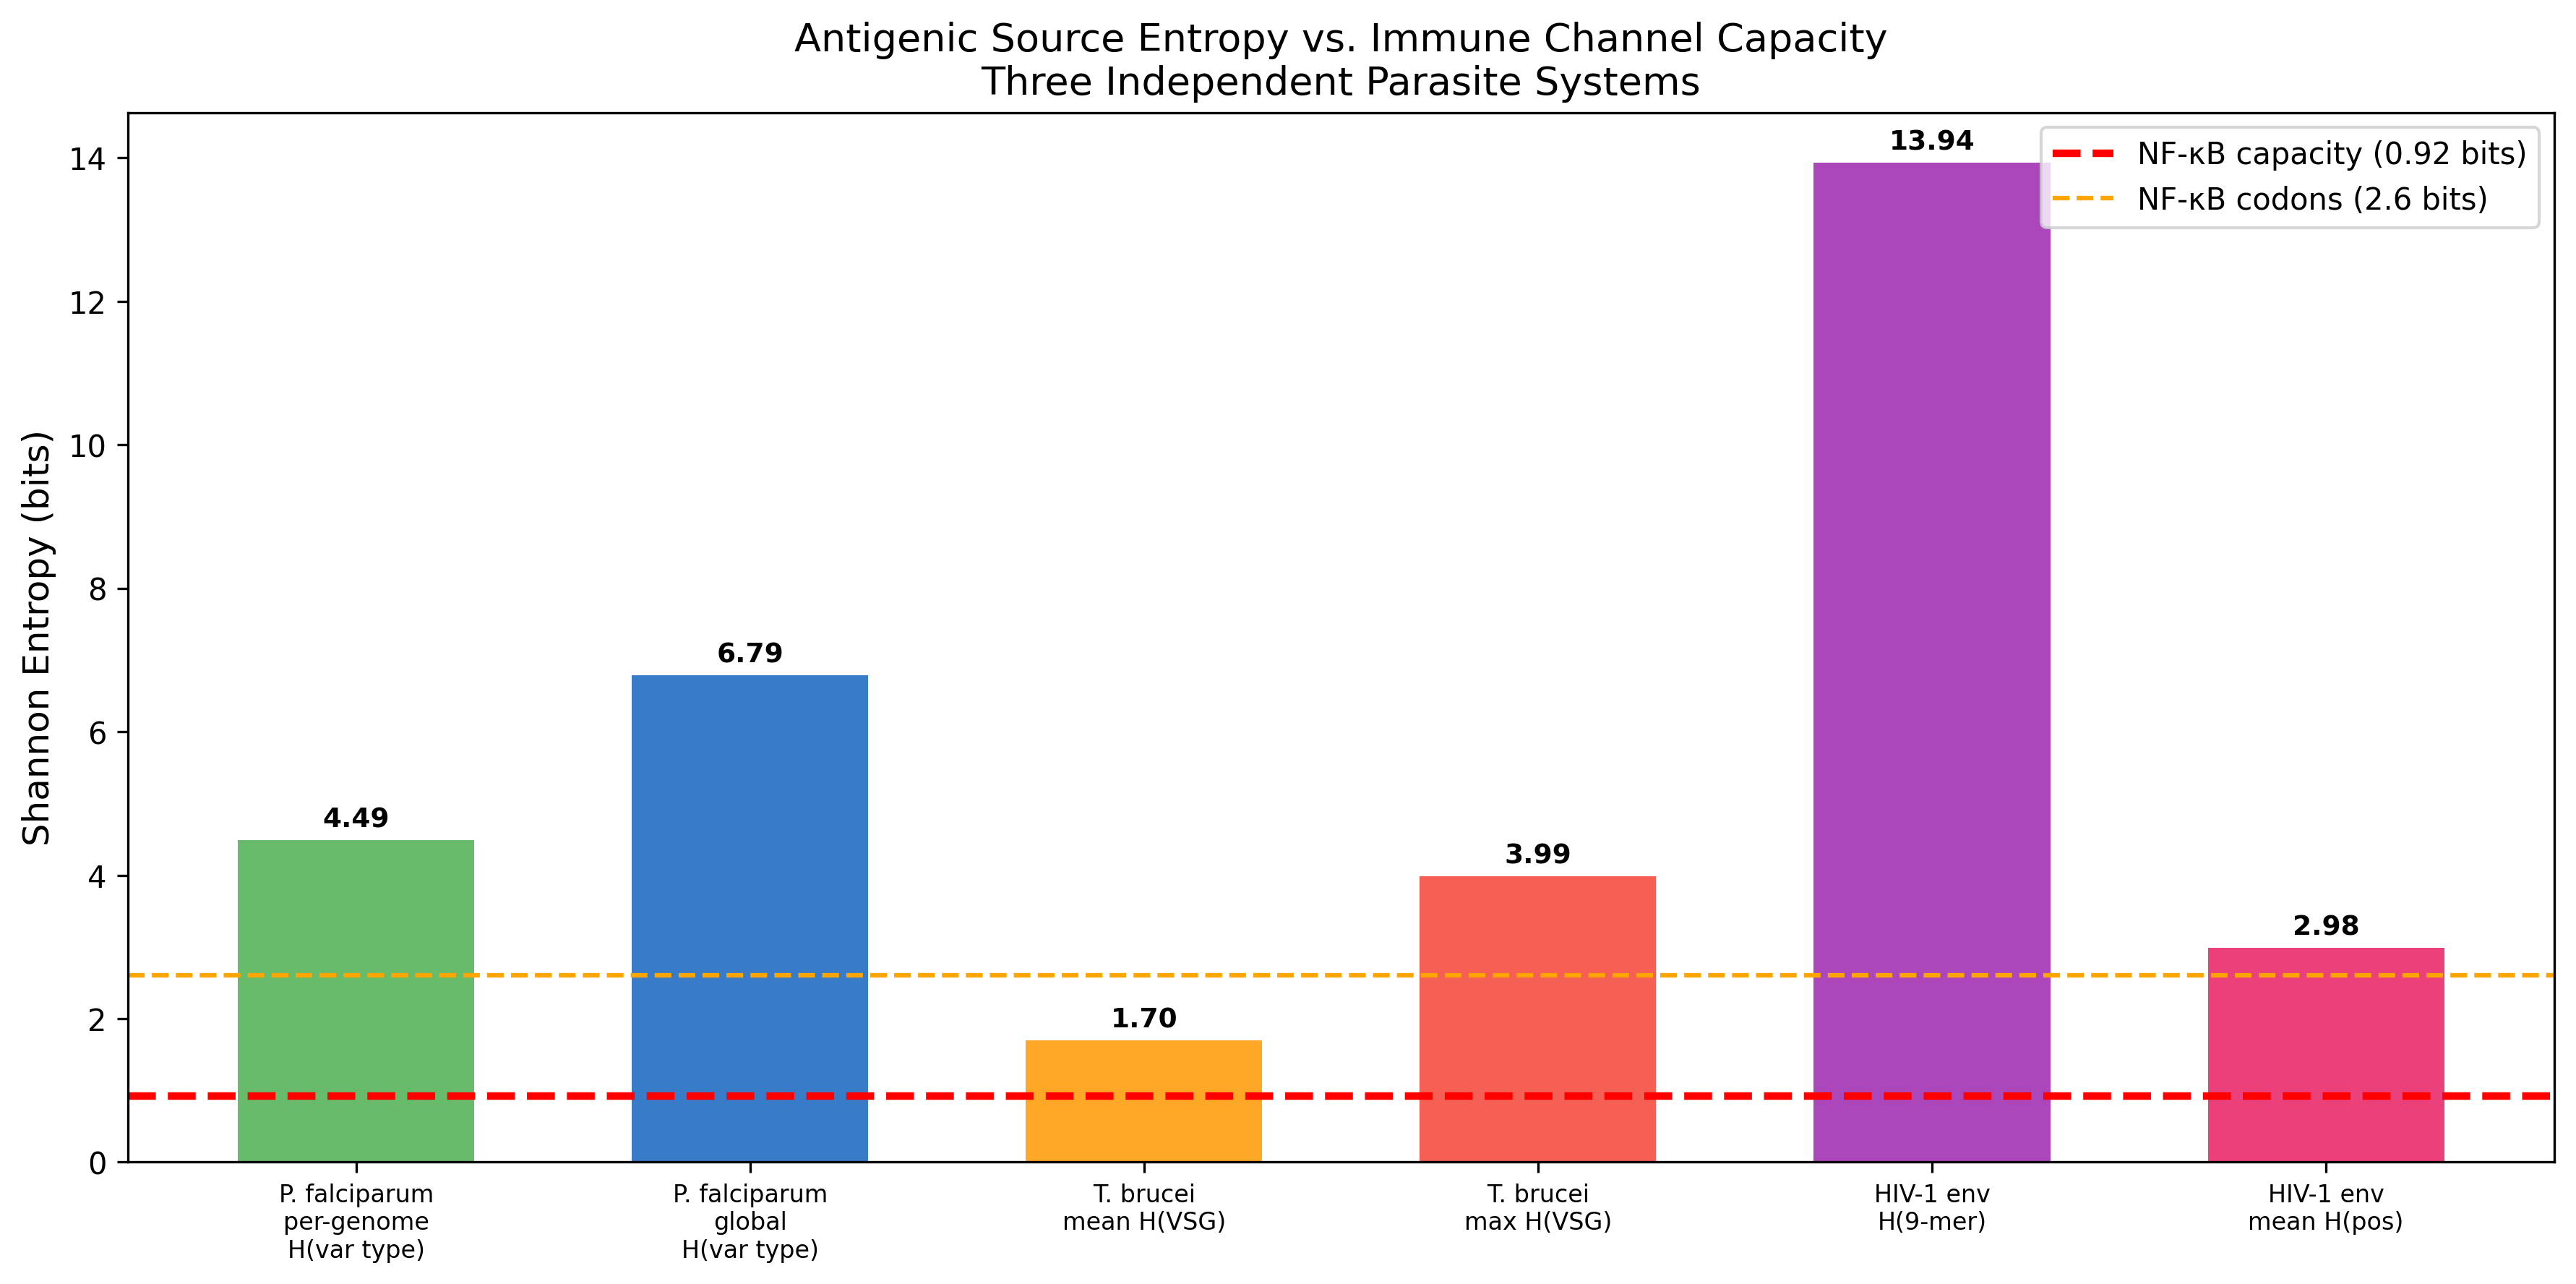
\includegraphics[width=\columnwidth]{figures/fig9_three_systems_summary.png}
\caption{Antigenic source entropy vs.\ immune channel capacity across three independent parasite systems.  All systems exceed the per-interaction capacity benchmark at every resolution level analyzed.  Dashed lines: published NF-$\kappa$B capacity measurements.}
\label{fig:summary}
\end{figure}

The minimum ratio across all analyses is $1.6\times$ (\textit{T.~brucei} Mouse~3 mean).  Even the most conservative resolution (\textit{P.~falciparum} first-domain-only, 18 types) gives $H/C = 2.2\times$.

% ============================================================
% 6. WHY H > C?
% ============================================================
\section{Why $H > C$ Across Three Unrelated Lineages?}
\label{sec:why}

\subsection{The Finding Is Arithmetic, Not Pattern-Seeking}

The finding is arithmetic, not interpretive.  We computed $H(X) = -\sum P(x) \log_2 P(x)$ on 168,738 var gene domain architectures and compared the result to $C = 0.92$~bits, a published measurement.  The inequality $6.79 > 0.92$ is a number exceeding another number, both computed using standard methods on peer-reviewed data.  The convergence across three systems does not reflect cherry-picking: we selected three canonical antigenically varying parasites \emph{a priori}---the textbook cases---and all three exceeded the benchmark.

What requires interpretation is \emph{why} three phylogenetically unrelated lineages---\textit{Plasmodium} (Apicomplexa), \textit{Trypanosoma} (Kinetoplastida), and HIV (Retroviridae)---independently converge on $H > C$.  Three frameworks offer complementary explanations:

\textbf{Framework 1: Shannon's converse theorem.}  If the immune channel has capacity $C$ and the parasite presents antigenic entropy $H > C$, reliable discrimination is impossible.  Our data shows $H/C$ ratios of 1.8--15.1$\times$ across three systems.  The immune system is in the $R > C$ regime.

\textbf{Framework 2: AVC theory.}  The Csisz\'{a}r-Narayan dichotomy theorem establishes that an adversary can drive channel capacity to zero if it can achieve symmetrizability.  Antigenic variation is a strategy toward symmetrizability---by expanding the antigenic alphabet beyond the channel's discriminative capacity, the parasite makes any given variant indistinguishable from others in the immune system's ``codebook.''

\textbf{Framework 3: Evolutionary game theory.}  The AVC's minimax structure---$\max_{P(X)} \min_{q(S)} I(X;Y)$ for the immune system, $\min_{q(S)} \max_{P(X)} I(X;Y)$ for the parasite---is proven equivalent to a zero-sum game~\citep{gallager1968,vonneumann1928}.  The saddle-point solution is the Nash equilibrium of this game.  \citet{bergstrom2005} proved that the fitness payoff of this game is the mutual information itself.  Natural selection, which is formally equivalent to the Multiplicative Weight Updates Algorithm~\citep{chastain2014}, converges on the minimax strategy.  The parasite \emph{will} find the capacity-exceeding antigenic diversity if the genetic repertoire permits it.

\subsection{The Channel Creates the Selection Pressure}

The broader implication is that the \emph{selection pressure} toward exploitation is a mathematical property of the channel's existence, not a biological contingency.  Any system that transmits information through a channel with positive capacity creates a fitness landscape where adversarial exploitation is rewarded.

However, a third condition determines whether any \emph{specific} organism realizes the strategy: \textbf{contingent feasibility}.  The organism must possess the genetic architecture to generate sufficient antigenic diversity, and the fitness benefit must exceed the metabolic cost.  \textit{T.~brucei} devotes ${\sim}10\%$ of its total protein synthesis to a single VSG coat~\citep{pays2004}, and maintains ${\sim}2{,}500$ VSG genes---a substantial genomic burden.  The strategy is expensive.  Not all parasites can afford it, and not all fitness landscapes lead to it.

The independent evolution of capacity-exceeding antigenic strategies in three unrelated lineages is evidence for \emph{strong convergent selection}, not for inevitability in the deterministic sense.  The $H > C$ strategy is one solution to the host-parasite evolutionary game---a prominent one, an effective one, and one that three major lineages independently discovered---but not the only one.

% ============================================================
% 7. DISCUSSION
% ============================================================
\section{Discussion}
\label{sec:discussion}

\subsection{What the Numbers Mean---and What They Do Not}

Our headline finding---parasitic antigenic entropy exceeds immune channel capacity by 1.8--15.1$\times$ at the per-interaction level---rests on standard computations applied to published data.  The entropy comes from genomic frequency distributions; the capacity from single-cell experiments.  The inequality $H > C$ is arithmetic.

The \emph{interpretation} of this inequality requires care.  It means:
\begin{enumerate}
\item \textbf{The immune system cannot simultaneously discriminate all variants.}  At $C = 0.92$~bits, the immune channel can distinguish $2^{0.92} \approx 1.9$ categories per signaling event.  A parasite presenting $2^{4.49} \approx 22.5$ variants per genome (for \textit{P.~falciparum}) overwhelms this capacity by an order of magnitude.
\item \textbf{Sequential learning partially compensates.}  The immune system is not limited to a single channel use.  Affinity maturation, memory cells, and repeated exposure allow the effective capacity to accumulate over time.  The relevant comparison is not just $H$ vs.\ $C$, but the rate of antigenic variation vs.\ the rate of immune learning.  The \textit{T.~brucei} oscillation data directly visualizes this race.
\item \textbf{Partial discrimination remains possible.}  Even a channel operating at $H/C = 5\times$ provides partial discrimination, reduces parasite load, and enables survival.  The 70\% channel efficiency of evolved molecular recognition systems~\citep{schneider2000} represents what evolution achieves under \emph{non-adversarial} noise.  Parasites represent adversarial noise---and the AVC literature shows that adversarial noise is fundamentally harder to cope with than stochastic noise.
\end{enumerate}

\subsection{The \textit{T.~brucei} Oscillation: A Real-Time Shannon Experiment}

The oscillating entropy trajectory in \textit{T.~brucei} infection (Section~\ref{sec:results}) is, to our knowledge, the most vivid empirical demonstration of Shannon capacity constraints in a biological system.  The alternation between low-entropy states ($H < C$, immune system discriminates, dominant variant cleared) and high-entropy states ($H > C$, immune system cannot discriminate, parasite diversifies) reproduces the fundamental phenomenology of a capacity-limited channel in real time.

This pattern was not predicted by our framework \emph{a priori}---we expected monotonic entropy increase.  The oscillation is more informative: it shows that the capacity constraint operates as a dynamic boundary around which the host-parasite arms race evolves.

\subsection{The Multi-Receiver Objection}

The strongest objection to our framework: the immune system comprises ${\sim}10^{11}$ cells operating in parallel, not a single NF-$\kappa$B wire.  A single-pathway capacity of 0.92~bits understates the system's aggregate discriminative power.

The answer depends on the correlation structure among immune cells.  Information theory provides two limiting regimes:

\textbf{Independent receivers (upper bound).}  If each of $M$ cells makes an independent observation, $C_{\text{aggregate}} = M \cdot C_{\text{single}}$.  For $M = 10^6$ responding cells, this gives ${\sim}10^6$~bits---vastly exceeding any parasitic entropy.

\textbf{Fully correlated receivers (lower bound).}  If all cells observe the same signal, $C_{\text{aggregate}} = C_{\text{single}} = 0.92$~bits regardless of $M$.

\textbf{The biologically relevant regime is intermediate.}  \citet{cheong2011} measured this directly: a population of ${\sim}14$ cells collectively achieves ${\sim}1.8$~bits---not $14 \times 0.92 = 12.9$~bits.  Capacity scales sublinearly, approximately as $C(M) \approx C_1 \cdot \log_2(M)$ where $C_1 \approx 0.23$~bits.  Extrapolating logarithmically: ${\sim}100$ cells yield ${\sim}1.5$~bits; ${\sim}1{,}000$ cells yield ${\sim}2.3$~bits; ${\sim}10^6$ cells yield ${\sim}4.6$~bits.

\begin{table}[t]
\centering
\caption{Multi-receiver capacity scaling: does $H > C$ survive?}
\label{tab:multi}
\footnotesize
\begin{tabular}{@{}lccl@{}}
\toprule
System & $H$ & $C_{\text{agg}}$ ($10^6$) & $H\!>\!C$? \\
\midrule
\textit{P.~f.} (global) & 6.79 & ${\sim}4.6$ & Yes \\
\textit{P.~f.} (per-genome) & 4.49 & ${\sim}4.6$ & Marginal \\
\textit{T.~b.} (mean) & 1.70 & ${\sim}4.6$ & No \\
\textit{T.~b.} (max) & 3.99 & ${\sim}4.6$ & No \\
HIV-1 (per-position) & 2.98 & ${\sim}4.6$ & No \\
HIV-1 (9-mer epitope) & 13.94 & ${\sim}4.6$ & Yes \\
\bottomrule
\end{tabular}
\smallskip

\footnotesize{$H$ and $C_{\text{agg}}$ in bits. Scaling: $C(M) \approx 0.23 \cdot \log_2(M)$.}
\end{table}

Under logarithmic scaling with $10^6$ coordinated cells, \textit{T.~brucei} mean VSG entropy and HIV per-position entropy fall \emph{below} the aggregate capacity.  The finding that $H > C$ at the per-interaction, single-pathway level is robust.  Whether it holds at the system level depends on the correlation structure among cells---which has been measured only for small populations (14 cells) and extrapolated here.

\begin{figure}[t]
\centering
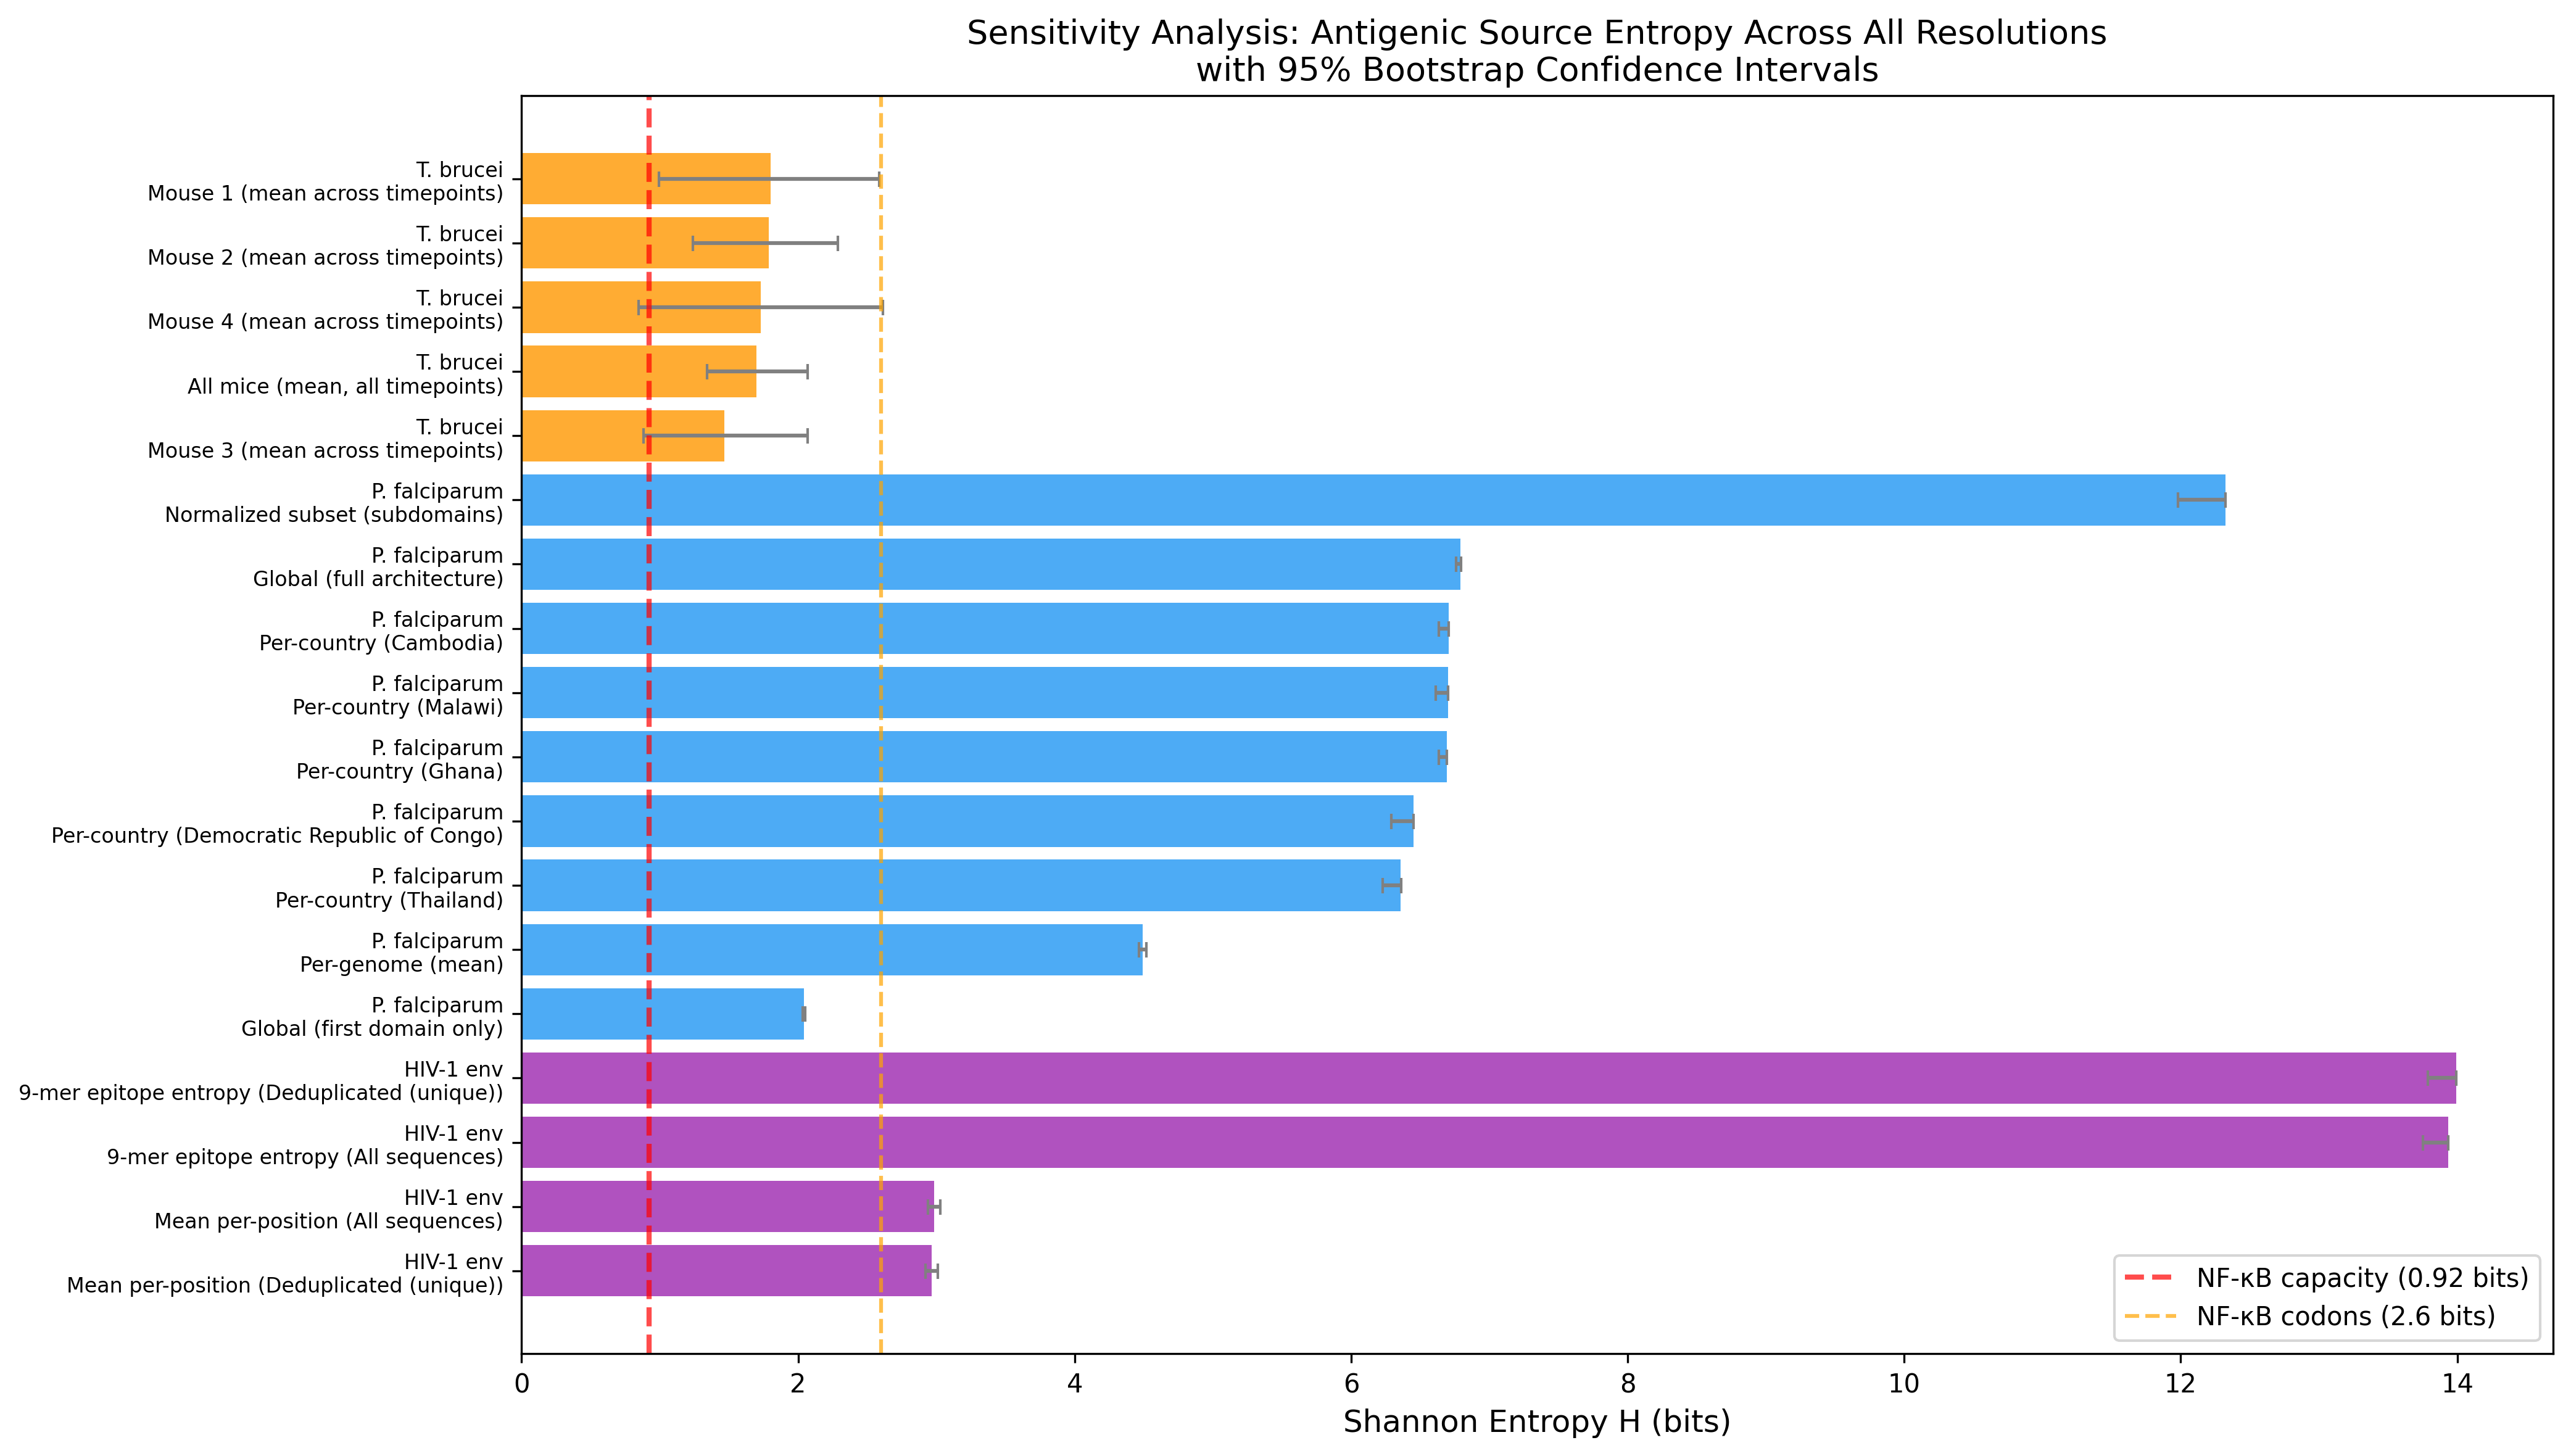
\includegraphics[width=\columnwidth]{figures/fig10_sensitivity_all_systems.png}
\caption{Sensitivity analysis: antigenic source entropy across all resolution levels with 95\% bootstrap confidence intervals.  Every measure exceeds the 0.92-bit NF-$\kappa$B capacity (red dashed line).  Blue: \textit{P.~falciparum}; orange: \textit{T.~brucei}; purple: HIV-1.}
\label{fig:sensitivity}
\end{figure}

Three considerations mitigate this concern.  First, the logarithmic extrapolation may itself be optimistic: not all $10^6$ cells encounter the same antigen simultaneously, and spatial and temporal delays reduce effective coordination.  Second, the HIV 9-mer entropy (13.94~bits) exceeds even aggressive aggregate estimates.  Applying Fano's inequality:
\begin{equation}
P_e \geq 1 - \frac{4.6 + 1}{13.94} \approx 0.60
\end{equation}
Even with $10^6$ coordinated cells, the minimum error probability for discriminating HIV 9-mer epitopes exceeds 60\%.  Against the single-pathway benchmark:
\begin{equation}
P_e \geq 1 - \frac{0.92 + 1}{13.94} \approx 0.86
\end{equation}
An 86\% minimum error probability at the single-cell level provides a quantitative explanation for why the cellular immune response fails to control HIV: the virus generates combinatorial diversity so vast that it overwhelms the recognition channel regardless of the capacity benchmark used.  Third, the \textit{T.~brucei} oscillation data provides direct empirical evidence that the capacity constraint binds \emph{in vivo}---clearance occurs only when entropy drops below ${\sim}1$~bit, consistent with a per-interaction capacity constraint.

\subsection{Rate of Antigenic Novelty vs.\ Rate of Immune Learning}

Shannon entropy of the antigenic repertoire measures \emph{source complexity} (a stock), not the rate at which antigens are presented to the immune system (a flow).  The proper comparison is between two rates:
\begin{equation}
R_{\text{novelty}} = \frac{dH(X)}{dt} \quad \text{vs.} \quad R_{\text{learning}} = \frac{dC_{\text{effective}}}{dt}
\end{equation}

Our \textit{T.~brucei} data provides the most direct measurement of $R_{\text{novelty}}$.  From the entropy trajectories across 4 mice, the observed entropy growth rate is ${\sim}0.04\text{--}0.06$~bits/day (linear fit to the upward-trending envelope of the oscillating trajectory).

Against this, the immune system's learning rate can be estimated from the kinetics of adaptive immunity.  A primary antibody response to a novel antigen requires ${\sim}7\text{--}14$ days~\citep{janeway2001}; affinity maturation requires ${\sim}2\text{--}3$ weeks; memory B-cell generation requires ${\sim}4\text{--}6$ weeks.  Each ``learning event'' adds ${\sim}1$ discriminable category to the immune codebook (i.e., ${\sim}1$~bit of capacity expansion).  This gives $R_{\text{learning}} \approx 0.07\text{--}0.14$~bits/day for the primary response.

The rates are approximately matched, consistent with the oscillation pattern: the parasite generates antigenic novelty at a rate slightly exceeding immune learning, maintaining the entropy above the per-interaction capacity threshold for most of the infection while the immune system periodically catches up (clearance events).  This rate-matching---rather than rate-domination---explains why trypanosome infections are chronic but not immediately lethal.  The parasite stays one step ahead, not ten steps ahead.

For HIV, the comparison is more extreme.  With a mutation rate of $3.4 \times 10^{-5}$ per nucleotide per replication cycle and ${\sim}10^{10}$ virions produced daily, HIV generates ${\sim}3.4 \times 10^5$ new nucleotide variants per day across the 2,600-nucleotide env gene.  The relevant immune learning rate---broadly neutralizing antibody development---requires years~\citep{haynes2012}.  Here $R_{\text{novelty}} \gg R_{\text{learning}}$, and the rate comparison reinforces rather than undermines the $H > C$ finding.

\subsection{Comparison to the Democratic Channel}

\citet{lopin2026} measured the channel efficiency of democratic preference-policy transmission at 2.7\% ($\eta = I(X;Y)/H(Y) = 0.025/0.934$).  \citet{schneider2000} measured molecular recognition efficiency at ${\sim}70\%$.  Both use Shannon's framework; both compare actual MI to theoretical capacity.

The parasitology findings complement these measurements by addressing channel \emph{degradation} rather than channel \emph{efficiency}.  The democratic channel operates at low efficiency due to institutional noise and capture.  Biological signaling channels operate at high efficiency under normal conditions (${\sim}70\%$) but are driven to low efficiency by adversarial parasitic exploitation.  The mathematical structure---$H_{\text{source}}$ vs.\ $C_{\text{channel}}$---is identical.

\subsection{Limitations}

\textbf{Channel capacity comparison is indirect.}  We compare parasitic source entropy to published immune channel capacity measurements, but these measurements were made in different experimental systems (mouse macrophages for NF-$\kappa$B, \emph{in vivo} human infections for antigenic variation).  The definitive test---measuring channel capacity in immune cells \emph{during} parasitic infection---has not been performed.

\textbf{Shannon entropy overstates effective diversity.}  Not all var genes or VSGs are equally immunogenic.  Functional constraints (cytoadherence for PfEMP1, receptor binding for VSG) reduce the effective antigenic space below the sequence-level diversity.  Amino acid substitutions in structurally buried positions are immunologically invisible; substitutions in epitope-facing surfaces are immunologically relevant.  Shannon entropy treats every distinct sequence as an equally informative symbol, ignoring this functional hierarchy.  Our entropy estimates are therefore \emph{upper bounds} on the immunologically relevant diversity.

However, three features of our analysis mitigate this concern.  First, we compute entropy over \emph{domain architectures} (combinations of DBL and CIDR domains) rather than raw sequences for \textit{P.~falciparum}.  Domain architecture determines both the antigenic surface and the binding phenotype---it is a functionally relevant classification, not a purely sequence-based one.  Second, our sensitivity analysis spans three orders of magnitude in classification granularity (18 first-domain types to 16,089 subdomain types), and the $H > C$ finding holds at every level---including the coarsest functional classification.  Third, for HIV, the concentration of per-position entropy at immune-facing surfaces (variable loops V1-V5: ${\sim}3.0\text{--}3.8$~bits) versus buried residues (conserved core: ${\sim}1.5\text{--}2.5$~bits) is itself evidence that the diversity is immunologically targeted rather than random.  The entropy is highest where the immune system looks hardest---precisely the pattern expected of evolved adversarial variation.

A more refined approach---computing ``functional information''~\citep{szostak2003} or ``effective antigenic entropy'' restricted to immunodominant epitopes---is a natural and important extension.  We note that such an approach would likely \emph{lower} our entropy estimates but \emph{also lower} the relevant capacity benchmark (since the immune system allocates most of its recognition capacity to immunodominant epitopes).  Whether the $H/C$ ratio increases or decreases under functional weighting is an empirical question we cannot resolve without paired antigen-response data.

\textbf{The DMC model is approximate.}  The immune system has memory (adaptive immunity), feedback (immune response modifies pathogen population), and non-stationarity (the channel changes over the course of infection).  These violate the discrete memoryless channel assumption.  The extensions required---channels with memory~\citep{verdu1994}, directed information~\citep{massey1990}, arbitrarily varying channels~\citep{csiszar1988}---are mathematically well-developed but have not been applied to host-parasite data.  We note these as natural extensions for future work.

However, the \textit{T.~brucei} oscillation data provides direct empirical evidence on how much compensation immune memory provides.  Memory B-cells and antibodies generated against previously dominant VSGs enable rapid clearance when those variants re-emerge---effectively ``caching'' decoded variants.  This caching is visible in the data: clearance events at days 18--24 occur faster than the initial response at days 6--12, consistent with memory-accelerated decoding.

But caching previously decoded variants does not help with \emph{novel} variants that the immune system has never encountered.  The oscillation pattern shows that after each clearance event, the parasite switches to new variants, entropy rises above the per-interaction capacity threshold, and the immune system must learn again from scratch for those new variants.  Memory provides \emph{temporal} capacity enhancement (faster re-recognition of known variants) but not \emph{bandwidth} enhancement (no improvement in discriminating among simultaneous novel variants).  The parasite's strategy---sequential deployment of novel variants from a large reservoir---is specifically adapted to exploit this distinction.  The reservoir ensures that the parasite always has variants the immune system has never seen, regardless of how many it has previously learned.

For channels with feedback (where the receiver's output affects the transmitter's future input), \citet{shannon1956} proved that feedback does not increase the capacity of memoryless channels.  For channels with memory, feedback \emph{can} increase capacity~\citep{coverpombra1989}.  The immune system's feedback (clearance of recognized variants selects for escape mutants) is precisely the scenario where feedback might increase effective capacity.  Quantifying this increase requires directed information analysis~\citep{massey1990} on paired temporal data of antigenic variation and immune response---a natural extension requiring longitudinal paired datasets that are not yet available.

\textbf{HIV cross-subtype inflation.}  Our HIV dataset spans multiple subtypes, inflating per-position entropy.  Single-subtype analysis would give lower but likely still capacity-exceeding values.

% ============================================================
% 8. CONCLUSION
% ============================================================
\section{Conclusion}
\label{sec:conclusion}

We have presented the first empirical measurement of parasitic immune evasion in Shannon's information-theoretic framework.  Three findings merit emphasis:

\begin{enumerate}
\item \textbf{All three parasite systems exceed immune channel capacity.}  \textit{P.~falciparum} antigenic entropy is 4.9--7.4$\times$ the NF-$\kappa$B capacity.  \textit{T.~brucei} VSG entropy averages 1.8$\times$ capacity, with peaks at 4.3$\times$.  HIV env positional entropy is 3.2$\times$ capacity, with 99.5\% of positions exceeding the benchmark.  The immune system operates in Shannon's $R > C$ regime.

\item \textbf{The \textit{T.~brucei} oscillation pattern is the Shannon limit made visible.}  VSG entropy oscillates above and below the ${\sim}1$-bit capacity threshold as the immune system clears dominant variants and the parasite switches.  This is, to our knowledge, the most direct empirical observation of a biological system crossing back and forth across a Shannon capacity boundary.

\item \textbf{Channel degradation is evolutionarily favored.}  The AVC theorem establishes that any channel with positive capacity \emph{can} be driven to zero capacity by a sufficiently powerful adversary.  Evolutionary game theory establishes that natural selection exerts pressure toward capacity-defeating strategies when the genetic architecture permits them.  The independent evolution of $H > C$ strategies in three phylogenetically unrelated lineages is consistent with strong convergent selection pressure.  The claim is not that every parasite \emph{must} evolve antigenic variation, but that those which do are driven toward the $H > C$ regime---and the three major lineages that have been studied all arrived there.
\end{enumerate}

The contribution is threefold.  First, connecting two mature literatures---immune signaling channel capacity and parasitic antigenic variation---that have developed independently for over a decade.  Second, providing quantitative measurements in bits that complement four decades of game-theoretic modeling of host-parasite coevolution.  Third, addressing the principal objection---that the immune system's aggregate, adaptive capacity exceeds single-pathway measurements---by deriving multi-receiver bounds, formalizing the rate-of-novelty versus rate-of-learning comparison, and showing that the \textit{T.~brucei} oscillation data provides direct \emph{in vivo} evidence that the per-interaction capacity constraint binds.

Two extensions constitute natural next steps.  First, measuring immune channel capacity \emph{during} parasitic infection---replicating the \citet{cheong2011} protocol in \textit{Toxoplasma}-infected macrophages or \textit{Plasmodium}-exposed immune cells.  This would transform the indirect comparison ($H_{\text{source}}$ vs.\ $C_{\text{published}}$) into a direct measurement of parasitic capacity degradation in bits.  Second, computing mutual information between antigenic variation and immune response using paired antigen-immunity datasets, which would measure not just source entropy but actual channel throughput under parasitic attack.

Every channel is a vulnerability---not because exploitation is inevitable, but because the selection pressure toward it is a mathematical property of the channel's existence.  The immune system is a channel.  Three unrelated lineages of parasites have independently discovered the proof.

% ============================================================
% DATA AND CODE AVAILABILITY
% ============================================================
\section*{Data and Code Availability}

Analysis code and processed data are available at \url{https://github.com/novalis78/Parasitology-Information-Theory}.  \textit{P.~falciparum} var gene data from \citet{otto2019} via Zenodo (doi:10.5281/zenodo.3549732).  \textit{T.~brucei} VSG-seq data from \citet{mugnier2015} via supplementary databases and GitHub (github.com/mugnierlab).  HIV-1 env sequences from NCBI Protein Database.  All results can be reproduced using the analysis scripts included in the repository.

% ============================================================
% ACKNOWLEDGMENTS
% ============================================================
\section*{Acknowledgments}

The author thanks the developers of the varDB database (Thomas Otto and colleagues), the Mugnier laboratory for making VSG-seq data publicly available, and the NCBI for programmatic access to HIV sequence data.  The information-theoretic framework was developed independently; any errors in its application are the author's own.

% ============================================================
% REFERENCES
% ============================================================
\bibliography{references}

\end{document}
